\section{Sample and observations}
\label{sec:obs}

We present multi-epoch optical and near-infrared spectroscopy of \Ntotal
carbon-sequence Wolf-Rayet (WC/WO) stars in the Large Magellanic Cloud,
obtained as part of ESO observation programme \esoProgrammes
(PI: T.\,Shenar) under VLT cycles P105--P107. Each target was observed
in \Nepochs epochs, distributed in service mode across three consecutive
semesters, for a total of \Ttotalhrs\,h of awarded VLT time. The cadence
and signal-to-noise targets were tailored to the dual goal of detecting
spectroscopic binaries among nominally single WC stars and of constraining
their underlying orbital period distribution.

\subsection{Target sample}
\label{sec:sample}

Our sample consists of \Ntotal WC- and WO-type Wolf-Rayet stars in the
Large Magellanic Cloud, drawn from the catalogue of
\citet{Breysacher1999} and the survey of \citet{Bartzakos2001}. Of these,
\Nknown were previously identified as spectroscopic binaries by
\citet{Bartzakos2001}; the remaining \Nstars stars were classified as
apparently single and form the primary targets of our survey.
Table~\ref{tab:sample} lists the target stars with their designations,
spectral types, and number of observed epochs. To balance signal-to-noise
requirements against the available VLT time, the sample was stratified
by apparent brightness into \Nbright bright targets ($V < 15$) and
\Nfaint faint targets ($V > 15$), each of which was assigned a distinct
exposure-time and observing-condition strategy (Sect.~\ref{sec:xshooter}).

\begin{figure}
\centering
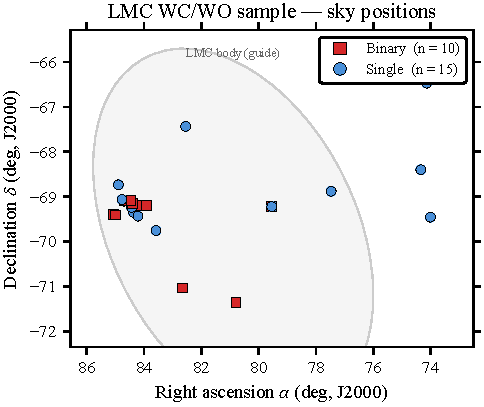
\includegraphics[width=\columnwidth]{plots/sample_map.pdf}
\caption{Sky positions of the \Ntotal LMC WC/WO targets overlaid on an
  H$\alpha$ image of the Large Magellanic Cloud. The \Nstars apparently
  single targets analysed in this work are shown in blue; the \Nknown
  previously known binaries from \citet{Bartzakos2001} are shown in
  orange.}
\label{fig:sample_map}
\end{figure}

\subsection{VLT/X-SHOOTER spectroscopy}
\label{sec:xshooter}

Multi-epoch spectroscopy was obtained with the X-SHOOTER spectrograph
\citep{Vernet2011} mounted on UT2 (Kueyen) of the ESO Very Large
Telescope at Cerro Paranal, Chile. X-SHOOTER is a three-arm
cross-dispersed echelle providing simultaneous wavelength coverage
across the UVB ($\sim 300$--$560$\,nm), VIS ($\sim 560$--$1020$\,nm),
and NIR ($\sim 1020$--$2480$\,nm) arms. We adopted slit widths of
\slitUVB in the UVB arm, \slitVIS in the VIS arm, and \slitNIR in the
NIR arm, yielding
an intermediate resolving power of $R \sim$ \Rxshooter across the full
wavelength range.

The choice of X-SHOOTER is motivated by two requirements specific to
the spectroscopic identification of WR binaries. First, the broad
emission lines that dominate WC spectra have full widths at half maximum
of order $10^{3}$\,\kms; resolving radial-velocity shifts at the few-\kms
level against this intrinsic width demands a spectral resolution of at
least $R \sim 5\,000$--$10\,000$, as established by previous WR binary
surveys \citep[e.g.][]{Bartzakos2001,Dsilva2022}.
Second, disentangling the WR component from a putative OB-type companion
benefits decisively from a multi-wavelength baseline: characteristic He,
C, and O features are distributed throughout the optical and near-infrared,
and the simultaneous arm-by-arm coverage delivered by X-SHOOTER provides
the broad spectral grasp required to track these features in a single
exposure. X-SHOOTER on the VLT uniquely satisfies both criteria for our
target brightness regime in the LMC.

A further motivation for broad coverage is the well-known sensitivity of
single-line WR radial velocities to wind variability and clumping:
estimates derived from a single emission line are biased by stochastic
line-profile variations of order $10$--$30$\,\kms. Cross-correlating across the eleven distinct He/C/O
emission lines listed in Table~\ref{tab:emission_lines}
(Sect.~\ref{sec:ccf}) averages down this stochastic component and brings
the per-epoch radial-velocity uncertainty into the few-\kms regime,
matching the precision required to detect long-period WR binaries.

The \Nepochs epochs per target were distributed as a 2$+$2$+$2 cadence
across the three observing semesters P105--P107, providing baselines
that range from days to ${\sim}\,500$\,d. This pattern was designed to
retain sensitivity to orbital periods up to $P \sim 10^{3}$\,d for
binaries whose RV semi-amplitudes exceed
$\Delta\mathrm{RV} \approx 30$\,\kms. The signal-to-noise and observing
conditions requested for the two brightness groups differ accordingly.
For the \Nbright bright targets, exposures were configured to reach
$\mathrm{S/N} \geq \snrTarget$ at $450$\,nm under airmass $\leq 2.2$,
seeing $\leq 1.3\arcsec$, and full lunar illumination. For the
\Nfaint faint targets, the requested S/N at $450$\,nm was relaxed to
${\sim}\,50$ but observing conditions were tightened to airmass
$\leq 1.8$, seeing $\leq 1.0\arcsec$, and lunar illumination
$\leq 0.5$, in order to keep the per-epoch read-noise contribution
sub-dominant relative to wind variability.

\subsection{Data reduction}
\label{sec:reduction}

Raw two-dimensional X-SHOOTER frames were reduced with the ESO
X-SHOOTER pipeline, which performs bias subtraction, flat-fielding,
order tracing, sky subtraction, wavelength calibration against ThAr arc
exposures, and flux calibration against spectrophotometric standards,
producing wavelength- and flux-calibrated 2D and 1D spectra per arm.
The subsequent post-processing --- spectral combination, continuum
normalisation, and (where necessary) spatial contamination removal ---
was performed using two custom tools developed for this work, both to
be released as open-source repositories upon publication. The full
post-processing chain is: an initial three-arm stitch
(Sect.~\ref{sec:stitch_initial}); continuum normalisation
(Sect.~\ref{sec:normalisation}); spatial contamination removal applied
arm-by-arm where needed (Sect.~\ref{sec:contamination_removal}); and a
final re-stitch of the cleaned, already-normalised arms into a single
1D per-epoch spectrum (Sect.~\ref{sec:stitch_final}).

\subsubsection{Initial spectral combination}
\label{sec:stitch_initial}

The three spectral arms were combined into a single working spectrum
per epoch using signal-to-noise-squared weighting. In the overlap
regions between adjacent arms, we computed the mean flux in the last
$5\%$ of the overlap for the redder arm and the corresponding region
of the bluer arm, deriving an alignment factor
$A = \bar{F}_\mathrm{red} / \bar{F}_\mathrm{blue}$. The two arms were
considered consistent if
\begin{equation}
|\bar{F}_\mathrm{red} - \bar{F}_\mathrm{blue}| <
\frac{\sqrt{\sigma_\mathrm{red}^2 + \sigma_\mathrm{blue}^2}}{\sqrt{N}}.
\end{equation}
Where the spectral sampling differed (e.g.\ NIR at $0.04$\,nm
vs.\ VIS at $0.02$\,nm), the lower-resolution spectrum was linearly
interpolated onto the finer grid before combination. The combined flux
was computed as $F_\mathrm{comb} = \sum w_i f_i$ with weights
$w_i = \mathrm{SNR}_i^2 / \sum \mathrm{SNR}_i^2$. This initial 1D
combined spectrum per epoch serves as the working spectrum for
continuum-anchor selection (Sect.~\ref{sec:normalisation}).

\subsubsection{Continuum normalisation}
\label{sec:normalisation}

Continuum normalisation was performed with a custom interactive
normalisation tool developed for this work and to be released as an
open-source repository upon publication. Continuum anchor points were
placed by visual inspection in featureless regions of the spectrum,
deliberately avoiding emission and absorption features as well as
telluric residuals. The flux assigned to each anchor was the
iteratively $3\sigma$-clipped mean over a narrow wavelength window
centred on the anchor wavelength, which suppresses the influence of
cosmic rays, hot pixels, and weak unresolved features that would
otherwise displace the local continuum estimate.

The pseudo-continuum was constructed as a piecewise linear interpolation
between consecutive anchor wavelengths, and the observed spectrum was
then divided by this interpolation to yield the normalised flux. The
same anchor wavelengths were reused for all \Nepochs epochs of a given
star, which enforces an epoch-to-epoch consistent normalised continuum
and removes a known source of artificial radial-velocity scatter that
arises when each epoch is normalised independently. Because the anchors
are defined in wavelength space, they can be reapplied unchanged to the
cleaned per-arm spectra produced by the contamination-removal step
(Sect.~\ref{sec:contamination_removal}); this means that no second pass
of anchor placement is required on the re-stitched spectrum
(Sect.~\ref{sec:stitch_final}).

\subsubsection{Spatial contamination removal}
\label{sec:contamination_removal}

In service-mode observations the X-SHOOTER slit can capture, in addition
to the WR target, a serendipitous source projected along the line of
sight that is \emph{not} a binary companion of the WR star --- for
example, an unrelated foreground or background star whose spatial
profile happens to fall within the slit during the exposure. If left
untreated, this contamination biases the 1D-extracted continuum and,
more critically, can imprint absorption features on the WR
emission-line profiles at overlapping wavelengths, mimicking or masking
genuine companion signatures.

To mitigate this, we developed a custom contamination-removal tool that
operates directly on the two-dimensional pipeline products, again to
be released as an open-source repository upon publication. The
identification of the WR's spatial position on the slit is unambiguous
because the WR emission lines are themselves localised tracers of the
WR's row in the spatial direction: their flux is strongly peaked at the
WR's spatial profile centre, and the \primaryline complex in particular
shows up as a bright vertical band in the 2D frame even when the
adjacent contaminant is comparable in continuum brightness.

The user manually selects, for each affected epoch, a spatial-direction
range that brackets the WR profile (typically a few arcseconds in
extent) and excludes the contaminating source. Only flux within this
range is collapsed along the spatial axis to produce the cleaned 1D
spectrum. The procedure is performed independently for each of the
three X-SHOOTER arms, so that the WR's spatial profile is delineated
on the actual 2D frame of each arm rather than inferred from one arm
and propagated to the others; this is important because the spatial
profile, slit illumination, and contaminant brightness ratio all vary
arm-to-arm. The output is one cleaned 1D spectrum per arm per affected
epoch. Stars showing no contamination in any arm are passed through
this step unchanged, with the user-selected spatial range covering the
full slit width, so that the workflow returns the standard pipeline
extraction in those cases.

\subsubsection{Final spectral combination}
\label{sec:stitch_final}

The cleaned per-arm 1D spectra are recombined into a single 1D
spectrum per epoch using the same signal-to-noise-squared weighting
and overlap-region alignment procedure described in
Sect.~\ref{sec:stitch_initial}. Because the continuum anchor wavelengths
defined in Sect.~\ref{sec:normalisation} are identical across all epochs
and are equally valid for the cleaned and uncleaned per-arm spectra,
the re-stitched spectrum is automatically normalised at the same
continuum points; no second round of anchor placement is required on
the final spectrum. The output is a single normalised, contamination-free
1D spectrum per star per epoch.

The resulting set of \Ntotal stars $\times$ \Nepochs epochs of normalised,
cleaned 1D spectra forms the input to the radial-velocity measurement
and binary classification pipeline described in Sect.~\ref{sec:methods}.
